\documentclass[11pt,a4paper]{article}
\usepackage{fontspec}
\renewcommand{\figurename}{Figura}\renewcommand{\tablename}{Tabela}\hyphenpenalty=10000 \exhyphenpenalty=10000 \tolerance=2000 \emergencystretch=3em
\setmainfont{Roboto}[Path=fonts/, Extension=.ttf, UprightFont=*-Regular, BoldFont=*-Bold, ItalicFont=*-Italic, BoldItalicFont=*-BoldItalic]
\setmonofont{lmmono10-regular.otf}[Scale=1.0]
\usepackage[a4paper, margin=2cm]{geometry}
\usepackage{xcolor}
\definecolor{titleblue}{HTML}{1E4E8C}
\definecolor{headfill}{HTML}{E8EEF7}
\definecolor{footgray}{HTML}{475569}
\definecolor{framegray}{HTML}{C9D1DB}
\definecolor{promptfill}{HTML}{F3F5F8}
\usepackage{graphicx}
\usepackage{array,tabularx,xltabular,colortbl}
\usepackage{enumitem}
\usepackage{titlesec}
\usepackage{fancyhdr}
\usepackage[labelsep=period,font={small,it},justification=centering]{caption}
\usepackage{float}
\usepackage{tikz}
\usetikzlibrary{positioning,arrows.meta,fit,backgrounds}
\usepackage[hidelinks]{hyperref}
\usepackage{xurl}
\usepackage{tcolorbox}
\tcbuselibrary{breakable}

\setlength{\parindent}{0pt}
\setlength{\parskip}{6pt}
\linespread{1.08}
\renewcommand{\arraystretch}{1.25}
\setlist[itemize]{label=\textbullet, leftmargin=1.4em, itemsep=3pt, topsep=4pt}

\titleformat{\section}{\color{titleblue}\Large\bfseries}{\thesection}{0.6em}{}
\titlespacing*{\section}{0pt}{14pt}{6pt}
\titleformat{\subsection}{\large\bfseries}{\thesubsection}{0.6em}{}
\titlespacing*{\subsection}{0pt}{12pt}{4pt}

\pagestyle{fancy}
\fancyhf{}
\renewcommand{\headrulewidth}{0pt}
\fancyfoot[L]{\small\color{footgray}UniBank · Grupo 7, Ponto e Vírgula · Atividade 2: Design de UX/UI e Prototipação}
\fancyfoot[R]{\small\color{footgray}\thepage}

\newcolumntype{L}[1]{>{\raggedright\arraybackslash}p{#1}}
\newcolumntype{Y}{>{\raggedright\arraybackslash}X}
\newcommand{\hd}[1]{\cellcolor{headfill}\textbf{#1}}
\newcommand{\cls}[1]{\texttt{#1}}
\newcommand{\telafig}[4]{%
  \begin{figure}[H]\centering\setlength{\fboxsep}{0pt}%
  \fcolorbox{framegray}{white}{\includegraphics[width=#2\linewidth]{img/#1.jpg}}%
  \caption{#3}\vspace{-2pt}%
  \begin{minipage}{\linewidth}#4\end{minipage}%
  \end{figure}}

\newcommand{\protolink}{https://igorbraziel.github.io/unibank-es/prototipo/}

\begin{document}

% ---------------- Capa ----------------
\begin{titlepage}
  \centering
  \vspace*{5cm}
  {\Huge\bfseries UniBank\par}
  \vspace{0.4cm}
  {\Large\color{titleblue} Sistema de gestão financeira integrado via Open Finance\par}
  \vspace{2.5cm}
  {\Large\bfseries Atividade 2: Design de UX/UI e Prototipação\par}
  \vspace{0.2cm}
  {\large Protótipo navegável das principais interfaces\par}
  \vfill
  {\large Grupo 7, Ponto e Vírgula\par}
  \vspace{0.4cm}
  Antônio Couto de Carvalho Júnior\\
  Miguel Venâncio Bertol\\
  Gustavo Bueno Ferreira\\
  Igor Reis Braziel\par
  \vspace{1.5cm}
  Engenharia de Software, Ciência da Computação (UFG)\\
  22 de outubro de 2026
\end{titlepage}
\setcounter{page}{1}

% ---------------- 1 ----------------
\section{Identificação da equipe e do sistema}

\begin{tabularx}{\linewidth}{|L{3.2cm}|Y|}
\hline
\hd{Equipe} & Grupo 7, Ponto e Vírgula \\ \hline
\hd{Integrantes} & Antônio Couto de Carvalho Júnior, Miguel Venâncio Bertol, Gustavo Bueno Ferreira e Igor Reis Braziel \\ \hline
\hd{Sistema} & UniBank \\ \hline
\hd{Objetivo} & Centralizar informações financeiras de diferentes instituições por meio do Open Finance, facilitando o controle de gastos, o planejamento e a tomada de decisões financeiras. \\ \hline
\hd{Atores} & Usuário final, administrador do sistema e instituições financeiras (sistemas externos). \\ \hline
\hd{Protótipo} & \url{\protolink} \\ \hline
\hd{Disciplina} & Engenharia de Software, Ciência da Computação (UFG) \\ \hline
\end{tabularx}

% ---------------- 2 ----------------
\section{Público-alvo}

O UniBank se destina a pessoas que possuem contas em diferentes instituições financeiras e desejam centralizar, organizar e acompanhar suas finanças em um único sistema. São, em geral, estudantes e profissionais que hoje alternam entre os aplicativos de cada banco e controlam os gastos em planilhas ou de memória, como levantado na elicitação de requisitos. O administrador do sistema é o usuário secundário, responsável pela auditoria e pelo monitoramento dos serviços.

\textbf{Persona de referência:} Ana Souza, 27 anos, analista em Goiânia. Tem conta corrente e cartão no Banco Aurora, conta corrente e poupança no Ipê Digital e uma conta na Cooperativa Cerrado. Para saber quanto tem, abre três aplicativos; os gastos em dinheiro ficam anotados numa planilha. As instituições citadas no protótipo são fictícias.

As principais necessidades do público-alvo orientaram as decisões de interface:

\begin{tabularx}{\linewidth}{|L{4.3cm}|Y|L{1.9cm}|}
\hline
\hd{Necessidade} & \hd{Decisão de interface} & \hd{Telas} \\ \hline
Ver a situação financeira completa rapidamente & O saldo em contas é o maior elemento do Início, com o saldo de cada conta logo abaixo. & T03 \\ \hline
Entender para onde vai o dinheiro & Gastos por categoria no Início, gráficos de pizza e de linha, e destaque para transações sem categoria no extrato. & T03, T04, T06 \\ \hline
Incluir gastos que o banco não registra & Botão \emph{Novo lançamento} no extrato, com formulário curto e validação junto aos campos. & T04, T05 \\ \hline
Confiar no compartilhamento de dados & Etapas numeradas, consentimento com dados, finalidade e prazo, aviso de que o UniBank não pede a senha do banco e confirmação antes de desconectar. & T09, T10, T11 \\ \hline
Não ser bloqueado pela falha de um banco & Avisos por instituição: as demais contas continuam disponíveis e a tela de falha indica a próxima ação. & T03, T08, T14 \\ \hline
(Administrador) Rastrear ações sensíveis e falhas de serviço & Logs somente leitura com filtros e status de cada serviço com o horário da última verificação. & T15, T16 \\ \hline
\end{tabularx}

% ---------------- 3 ----------------
\section{Fluxo principal de navegação}

\subsection{Estrutura de navegação}

O usuário final navega por cinco seções fixas: Início, Extrato, Gráficos, Relatórios e Minhas conexões. No computador, elas ficam no menu lateral; no celular, em uma barra inferior. O login é único: a operação \cls{autenticar} da classe \cls{Usuario} direciona o usuário final ao Início e o administrador às telas de Logs de auditoria e Status dos serviços. A Figura~\ref{fig:mapa} mostra todas as telas e as transições entre elas; o fluxo principal aparece destacado.

\begin{figure}[H]
\centering
\resizebox{\linewidth}{!}{%
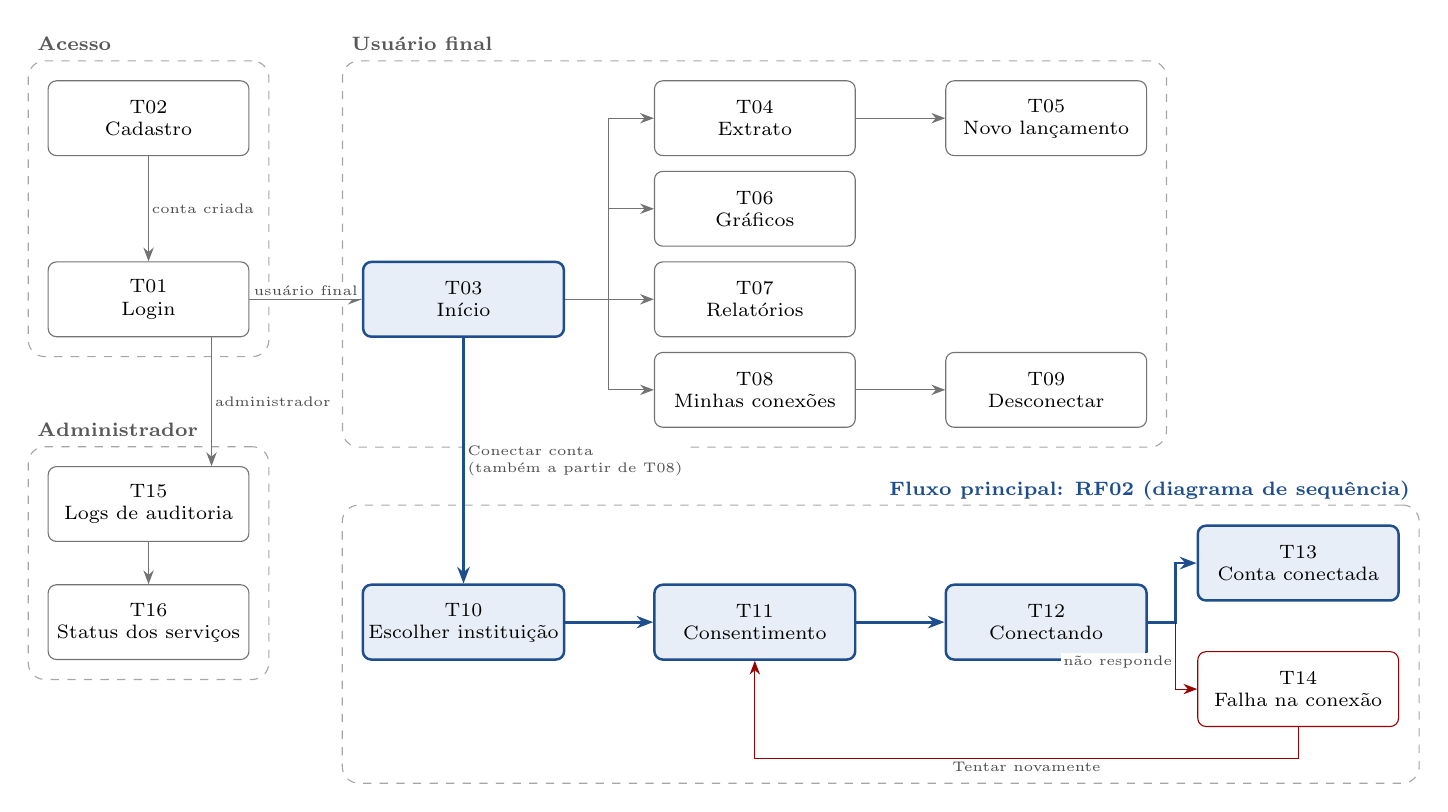
\begin{tikzpicture}[
  scr/.style={draw=black!55, rounded corners=3pt, fill=white, font=\scriptsize, align=center, minimum width=2.55cm, minimum height=0.95cm, inner sep=2pt},
  key/.style={scr, draw=titleblue, line width=0.9pt, fill=headfill},
  ar/.style={-{Stealth[length=5pt]}, black!55},
  kar/.style={-{Stealth[length=6pt]}, titleblue, line width=1pt},
  lbl/.style={font=\tiny, fill=white, inner sep=1pt, text=black!70},
  area/.style={draw=black!35, dashed, rounded corners=6pt, inner sep=7pt},
  atitle/.style={font=\scriptsize\bfseries, text=black!65, anchor=north west}
]
% Acesso e administrador
\node[scr] (t02) at (0,6.9) {T02\\Cadastro};
\node[scr] (t01) at (0,4.6) {T01\\Login};
\node[scr] (t15) at (0,2.0) {T15\\Logs de auditoria};
\node[scr] (t16) at (0,0.5) {T16\\Status dos serviços};
% Usuário final
\node[key] (t03) at (4.0,4.6) {T03\\Início};
\node[scr] (t04) at (7.7,6.9) {T04\\Extrato};
\node[scr] (t06) at (7.7,5.75) {T06\\Gráficos};
\node[scr] (t07) at (7.7,4.6) {T07\\Relatórios};
\node[scr] (t08) at (7.7,3.45) {T08\\Minhas conexões};
\node[scr] (t05) at (11.4,6.9) {T05\\Novo lançamento};
\node[scr] (t09) at (11.4,3.45) {T09\\Desconectar};
% Fluxo RF02
\node[key] (t10) at (4.0,0.5) {T10\\Escolher instituição};
\node[key] (t11) at (7.7,0.5) {T11\\Consentimento};
\node[key] (t12) at (11.4,0.5) {T12\\Conectando};
\node[key] (t13) at (14.6,1.25) {T13\\Conta conectada};
\node[scr, draw=red!60!black] (t14) at (14.6,-0.35) {T14\\Falha na conexão};

\draw[ar] (t02) -- node[lbl,right]{conta criada} (t01);
\draw[ar] (t01) -- node[lbl,above]{usuário final} (t03);
\draw[ar] ([xshift=0.8cm]t01.south) -- node[lbl,right]{administrador} ([xshift=0.8cm]t15.north);
\draw[ar] (t15) -- (t16);
\draw[ar] (t03.east) -- ++(0.55,0) |- (t04.west);
\draw[ar] (t03.east) ++(0.55,0) |- (t06.west);
\draw[ar] (t03.east) -- (t07.west);
\draw[ar] (t03.east) ++(0.55,0) |- (t08.west);
\draw[ar] (t04) -- (t05);
\draw[ar] (t08) -- (t09);
\draw[kar] (t03) -- node[lbl,right,align=left]{Conectar conta\\(também a partir de T08)} (t10);
\draw[kar] (t10) -- (t11);
\draw[kar] (t11) -- (t12);
\draw[kar] (t12.east) -- ++(0.35,0) |- (t13.west);
\draw[ar, red!60!black] (t12.east) ++(0.35,0) |- node[lbl, pos=0.3, left]{não responde} (t14.west);
\coordinate (low) at (8,-1.3);
\draw[ar, red!60!black] (t14.south) -- ++(0,-0.4) -| node[lbl, pos=0.25, below]{Tentar novamente} (t11.south);

\begin{scope}[on background layer]
\node[area, fit=(t02)(t01)] (a1) {};
\node[area, fit=(t15)(t16)] (a2) {};
\node[area, fit=(t03)(t04)(t05)(t08)(t09)] (a3) {};
\node[area, fit=(t10)(t11)(t12)(t13)(t14)(low)] (a4) {};
\end{scope}
\node[atitle] at ([yshift=12pt]a1.north west) {Acesso};
\node[atitle] at ([yshift=12pt]a2.north west) {Administrador};
\node[atitle] at ([yshift=12pt]a3.north west) {Usuário final};
\node[atitle, text=titleblue, anchor=north east] at ([yshift=12pt]a4.north east) {Fluxo principal: RF02 (diagrama de sequência)};
\end{tikzpicture}}
\caption{Mapa de navegação do protótipo. Em azul, o fluxo principal do RF02.}
\label{fig:mapa}
\end{figure}

\subsection{Fluxo principal: conectar conta via Open Finance (RF02, US02)}

O fluxo principal do protótipo é o mesmo do diagrama de sequência da Atividade 1. A tabela abaixo relaciona cada passo às telas e às mensagens do diagrama.

\begingroup\small
\begin{xltabular}{\linewidth}{|L{0.9cm}|L{2.7cm}|Y|L{5.3cm}|}
\hline
\hd{Passo} & \hd{Tela} & \hd{O que o usuário faz e vê} & \hd{Mensagens do diagrama} \\ \hline
\endhead
1 & T03 Início ou T08 Minhas conexões & Aciona \emph{Conectar conta}. & (início do fluxo) \\ \hline
2 & T10 Escolher instituição & Seleciona a instituição (Banco Horizonte) e aciona \emph{Continuar}. O botão só fica habilitado após a escolha. & 1 seleciona instituição; 2 \cls{conectarConta\allowbreak(instituicao)}; 3 \cls{solicitarAutorizacao\allowbreak(instituicao)} \\ \hline
3 & T11 Consentimento & No ambiente da instituição, revisa os dados compartilhados, a finalidade e o prazo, e aciona \emph{Autorizar compartilhamento}. & 4 pede consentimento; nota “o usuário autoriza o compartilhamento”; 5 token de acesso \\ \hline
4 & T12 Conectando & Acompanha o progresso: autorização recebida, busca das contas e conclusão da conexão. & 6 token; 7 \cls{criar(instituicao,\allowbreak token)}; 8 \cls{autorizar()}; 9 a 12 \cls{obterContas(c)}; 13 \cls{registrarLog(usuario, CONEXAO, sucesso)} \\ \hline
5 & T13 Conta conectada & Vê as contas encontradas e o novo saldo em contas. Ao voltar ao Início, a conta já aparece no saldo e no extrato. & 14 conta conectada; 15 exibe conta conectada \\ \hline
\end{xltabular}
\endgroup

\subsection{Fluxo alternativo: a instituição não responde}

Se a instituição não responde no passo 4, o protótipo exibe a tela T14 (mensagens 16 a 19 do fragmento \cls{alt}). A mensagem informa o que aconteceu, que nenhum dado foi compartilhado e que as demais conexões continuam funcionando (RNF04 e RNF08). O botão \emph{Tentar novamente} volta à etapa de consentimento. A tentativa é registrada nos logs como \cls{CONEXAO} com falha, o que pode ser conferido na tela T15. No protótipo, esse cenário é ativado pela opção \emph{Instituição não responde} do painel do protótipo (Seção~\ref{sec:link}).

\subsection{Fluxos secundários}

\begin{itemize}
\item \textbf{Cadastro e login (RF01):} T02 $\rightarrow$ T01 (com confirmação da conta criada) $\rightarrow$ T03.
\item \textbf{Extrato e lançamentos (RF04 a RF06):} T04 $\rightarrow$ T05 (diálogo de novo lançamento) $\rightarrow$ T04, com o lançamento já listado. A categoria é escolhida na própria linha do extrato.
\item \textbf{Análise (RF07 a RF09):} T03 $\rightarrow$ T06 (Ver gráficos) e T03 $\rightarrow$ T07 (Relatórios), com geração e exportação do relatório.
\item \textbf{Gestão das conexões (RF10 a RF12):} T08 $\rightarrow$ \emph{Atualizar dados}, \emph{Renovar consentimento} (que reutiliza o fluxo do RF02) ou T09 (confirmação de desconexão) $\rightarrow$ T08.
\item \textbf{Administração (RF13 e RF14):} T01 $\rightarrow$ T15 $\rightarrow$ T16.
\end{itemize}

% ---------------- 4 ----------------
\section{Telas do protótipo}

\subsection{Identidade visual e princípios de UX/UI}

A identidade visual usa verde-petróleo como cor principal, para transmitir segurança, e amarelo-ipê como destaque, em referência ao Cerrado. Os títulos e valores usam a fonte Bricolage Grotesque e os textos, a IBM Plex Sans, ambas do Google Fonts. O protótipo funciona no computador e no celular e acompanha o tema claro ou escuro do dispositivo. As etiquetas tracejadas no topo das telas (por exemplo, \emph{T03 · RF03, RF07}) identificam a tela e os requisitos atendidos; elas existem apenas no protótipo e podem ser ocultadas.

\begin{tabularx}{\linewidth}{|L{3.4cm}|Y|}
\hline
\hd{Princípio} & \hd{Aplicação no protótipo} \\ \hline
Hierarquia visual & O saldo em contas é o maior elemento do Início. Os totais aparecem antes do detalhe, como no extrato e nos relatórios. \\ \hline
Consistência & Menu, cabeçalho de página, botões (primário preenchido, secundário contornado, destrutivo em vermelho) e selos de status são os mesmos em todas as telas. \\ \hline
Legibilidade & Rótulos visíveis em todos os campos, valores com algarismos alinhados, contraste adequado nos temas claro e escuro. \\ \hline
Facilidade de navegação & Cinco seções fixas, etapas numeradas no fluxo de conexão e atalhos contextuais, como \emph{Ver extrato} e \emph{Categorizar no extrato}. \\ \hline
Feedback das ações & Mensagens após salvar, categorizar, atualizar, exportar e desconectar; estados de carregamento; erros que explicam o problema e como resolver. \\ \hline
Prevenção de erros & Validação junto a cada campo, confirmação antes de desconectar, mensagem genérica no login (US01) e botão de continuar habilitado somente após a escolha da instituição. \\ \hline
Acessibilidade e responsividade & Navegação por teclado com foco visível, diálogos que fecham com Esc, cor sempre acompanhada de ícone e texto, e layout que se adapta ao celular. \\ \hline
\end{tabularx}

\subsection{Telas}

\telafig{T01_login}{0.84}{T01, Login (RF01).}{O login é único para o usuário final e para o administrador. Com credenciais incorretas, a mensagem não indica qual campo está errado, conforme o critério de aceitação da US01. O quadro tracejado é exclusivo do protótipo e preenche os acessos de demonstração.}

\telafig{T02_cadastro}{0.84}{T02, Cadastro (RF01, RNF02).}{Cada campo é validado individualmente, as regras de senha são conferidas enquanto o usuário digita e o cadastro exige o aceite dos Termos de Uso e da Política de Privacidade (LGPD). Depois de criar a conta, o usuário volta ao login com a confirmação.}

\telafig{T03_inicio}{0.6}{T03, Início (RF03, RF07, RNF03, RNF04, RNF06).}{O Início reúne o saldo em contas, o saldo de cada conta, o comparativo com o mês anterior, os gastos por categoria e as últimas movimentações, atendendo ao critério da US07. O aviso da Cooperativa Cerrado mostra que uma instituição com consentimento expirado não bloqueia as demais (RNF04).}

\telafig{T04_extrato}{0.84}{T04, Extrato (RF04, RF06).}{Cada movimentação mostra data, descrição, categoria, conta de origem e valor, da mais recente para a mais antiga (US04). A categoria é escolhida na própria linha, e as transações sem categoria ficam destacadas (US06). Lançamentos manuais aparecem como \emph{Lançamento manual}, isto é, uma \cls{Transacao} sem conta de origem.}

\telafig{T05_lancamento}{0.84}{T05, Novo lançamento manual (RF05).}{O diálogo pede tipo, valor, data, descrição e categoria opcional. Ao salvar, o lançamento aparece no extrato e entra nos totais do Início, conforme a US05.}

\telafig{T06_graficos}{0.66}{T06, Gráficos (RF09).}{A tela traz o gráfico de pizza de gastos por categoria, com a tabela de valores, e o gráfico de linha de receitas e despesas por mês (US09). Ao passar o cursor, o gráfico mostra os valores do mês. Despesas sem categoria são sinalizadas, pois o gráfico depende da categorização (US06).}

\telafig{T07_relatorios}{0.66}{T07, Relatórios (RF08).}{O usuário escolhe o período e recebe o resumo de receitas, despesas e saldo, além das despesas por categoria, com exportação em PDF ou CSV (US08). No protótipo, a exportação é simulada.}

\telafig{T08_conexoes}{0.84}{T08, Minhas conexões (RF10, RF11).}{Cada instituição mostra o status (Ativa ou Expirada), as contas, a validade do consentimento e a última atualização (US10). As ações permitem atualizar os dados (US11), renovar o consentimento expirado e desconectar.}

\telafig{T09_desconectar}{0.84}{T09, Desconectar instituição (RF12, RNF05).}{A confirmação explica o efeito da ação: o consentimento é revogado e as contas saem do painel. Ela também informa que a desconexão fica registrada no histórico de segurança (US12).}

\telafig{T10_conectar}{0.84}{T10, Escolher instituição (RF02, mensagem 1).}{Primeira etapa do fluxo principal: etapas numeradas, busca por nome, instituições já conectadas desabilitadas e uma explicação de como a conexão funciona.}

\telafig{T11_consentimento}{0.84}{T11, Consentimento na instituição (RF02, RNF02, mensagens 4 e 5).}{Tela simulada do ambiente da instituição, com os dados compartilhados, a finalidade e o prazo do consentimento, como no Open Finance Brasil. O usuário pode recusar ou autorizar.}

\telafig{T12_conectando}{0.84}{T12, Conectando (RF02, mensagens 6 a 13).}{O progresso é exibido em três etapas enquanto o sistema cria a conexão, obtém as contas e registra o log.}

\telafig{T13_conectada}{0.84}{T13, Conta conectada (RF02, mensagens 14 e 15).}{Fim do fluxo principal: a tela mostra as contas encontradas e o novo saldo em contas, com atalhos para o Início e para conectar outra conta.}

\telafig{T14_falha}{0.84}{T14, Falha na conexão (RF02, RNF04, RNF08, mensagens 16 a 19).}{Fluxo alternativo: a mensagem é clara, informa que nenhum dado foi compartilhado e que as outras conexões continuam funcionando, e oferece \emph{Tentar novamente}.}

\telafig{T15_logs}{0.84}{T15, Logs de auditoria (RF13, RNF05).}{Os registros mostram usuário, ação, data e hora e resultado, são somente leitura e podem ser filtrados (US13). As ações feitas durante a navegação no protótipo também aparecem na lista.}

\telafig{T16_servicos}{0.84}{T16, Status dos serviços (RF14).}{Há um cartão para cada componente do diagrama de componentes, com o status e o horário da última verificação (US14). Na figura, a Integração Open Finance aparece indisponível, cenário ativado pelo painel do protótipo.}

\begin{figure}[H]
\centering
\setlength{\fboxsep}{0pt}
\fcolorbox{framegray}{white}{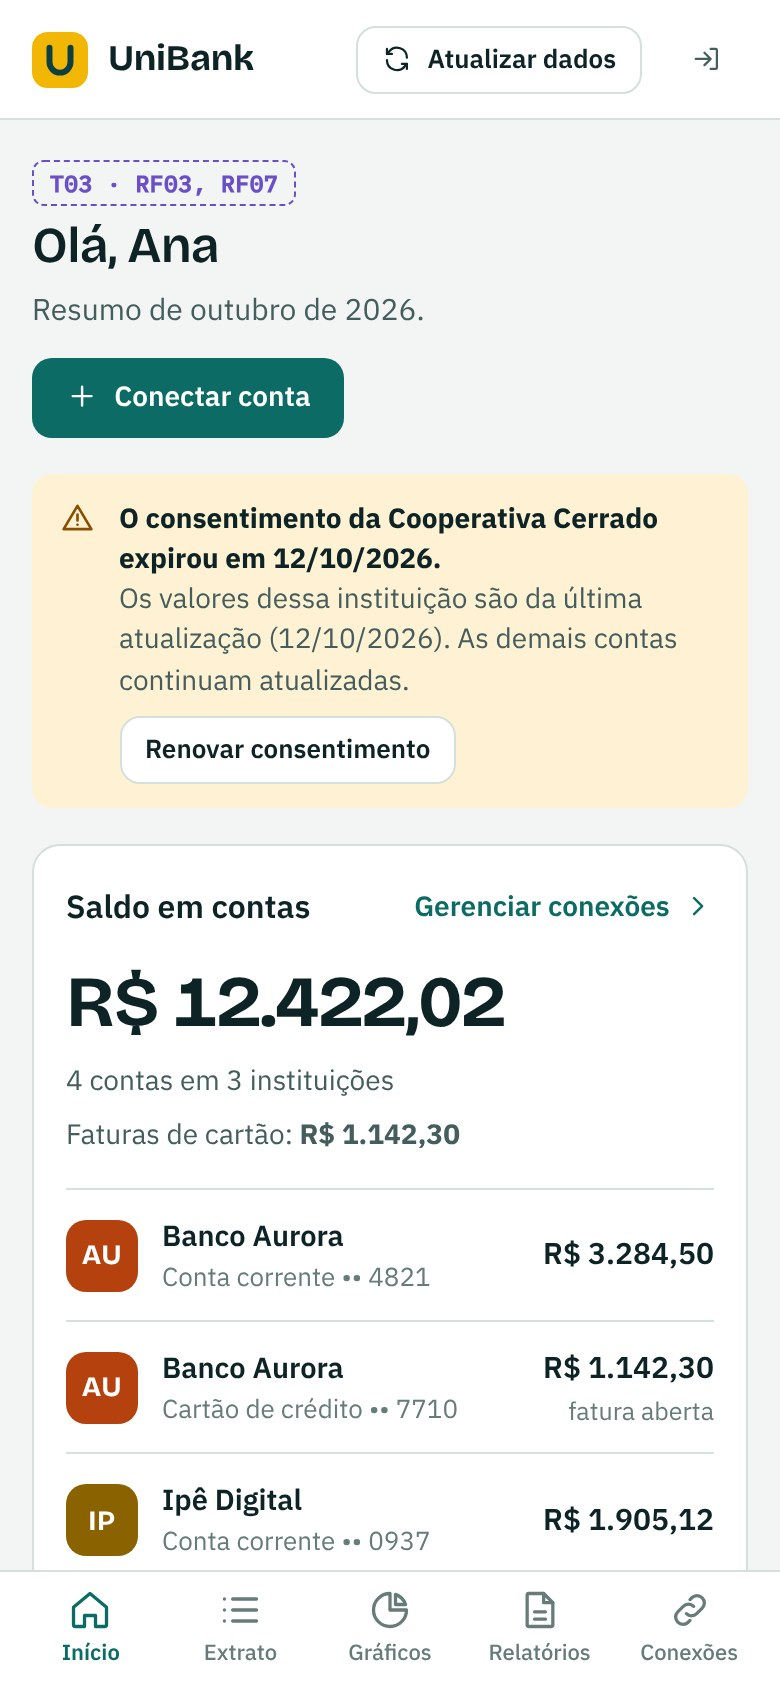
\includegraphics[width=0.25\linewidth]{img/M1_inicio.jpg}}\hfill
\fcolorbox{framegray}{white}{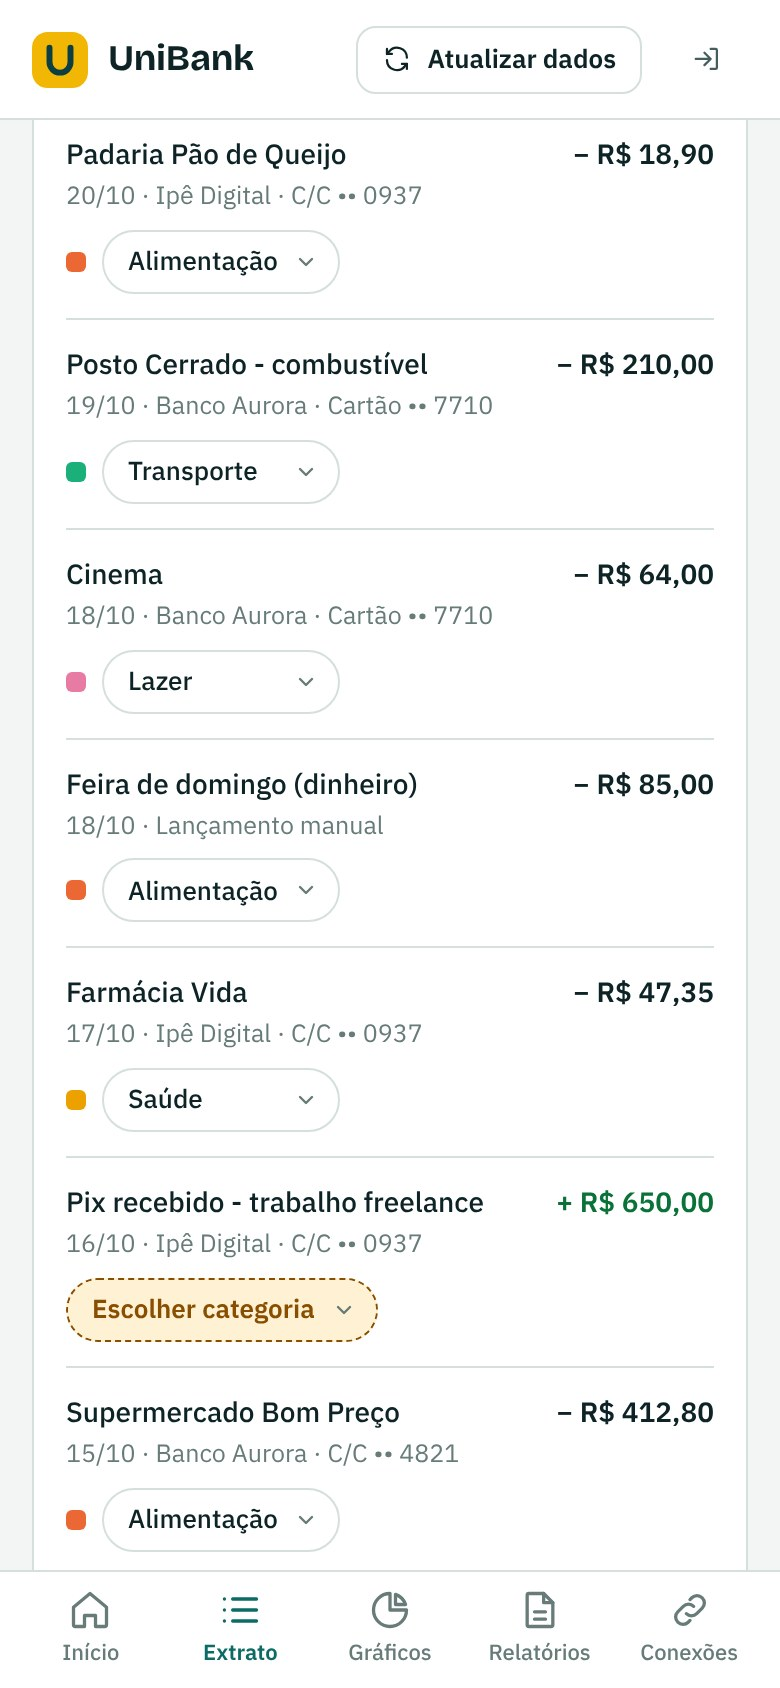
\includegraphics[width=0.25\linewidth]{img/M2_extrato.jpg}}\hfill
\fcolorbox{framegray}{white}{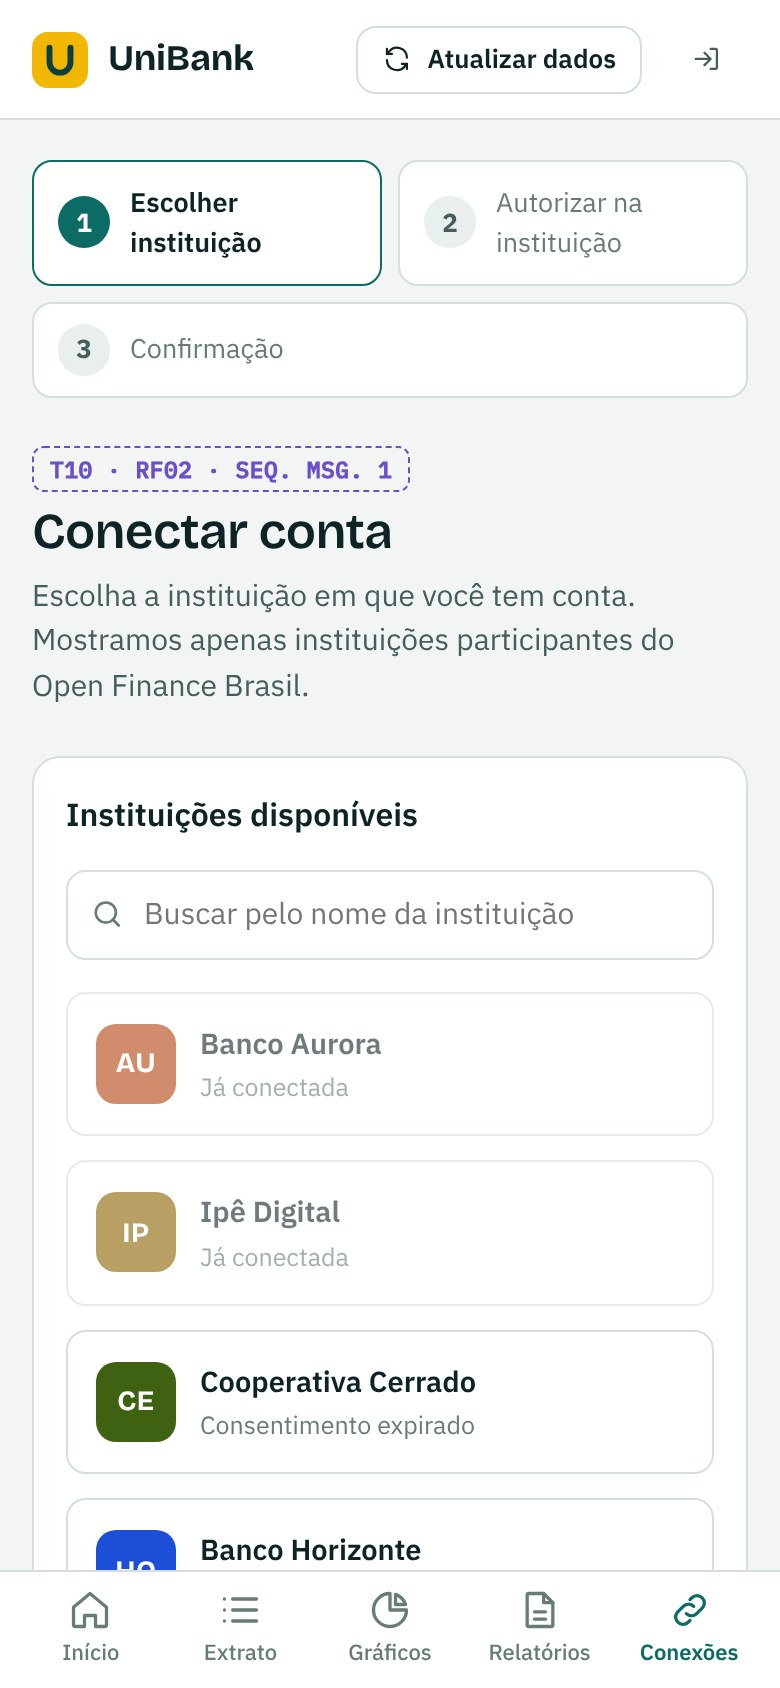
\includegraphics[width=0.25\linewidth]{img/M3_conectar.jpg}}
\caption{Início, Extrato e Escolher instituição em largura de celular.}\vspace{-2pt}
\begin{minipage}{\linewidth}No celular, o menu lateral vira uma barra inferior e a tabela do extrato vira uma lista, sem rolagem horizontal.\end{minipage}
\end{figure}

% ---------------- 5 ----------------
\section{Link de acesso ao protótipo}
\label{sec:link}

\textbf{Protótipo navegável:} \url{\protolink}

O protótipo abre em qualquer navegador, no computador ou no celular. Para percorrer o fluxo principal: \emph{Preencher usuário final} $\rightarrow$ \emph{Entrar} $\rightarrow$ \emph{Conectar conta} $\rightarrow$ \emph{Banco Horizonte} $\rightarrow$ \emph{Continuar} $\rightarrow$ \emph{Autorizar compartilhamento}.

O botão \emph{Mapa do protótipo}, no canto inferior direito, abre um painel que não faz parte do UniBank e apoia a avaliação:

\begin{itemize}
\item \textbf{Mapa de telas:} acesso direto às telas T01 a T16, com os requisitos de cada uma.
\item \textbf{Cenários:} \emph{Instituição não responde} (fluxo alternativo do RF02 e erro ao atualizar dados no RF11), \emph{Serviço fora do ar} (RF14) e exibição das etiquetas de identificação das telas.
\item \textbf{Acessos de demonstração:} usuário final \cls{ana.souza@email.com} / \cls{unibank123}; administrador \cls{admin@unibank.com.br} / \cls{admin123}.
\item \textbf{Restaurar dados de exemplo:} volta o protótipo ao estado inicial.
\end{itemize}

% ---------------- 6 ----------------
\section{Matriz de rastreabilidade atualizada}

\begingroup\small
\begin{xltabular}{\linewidth}{|L{2.8cm}|L{3.7cm}|L{2.6cm}|L{2.2cm}|Y|}
\hline
\hd{Requisito} & \hd{Classes (operações)} & \hd{Componentes} & \hd{Diagrama de Sequência} & \hd{Telas do protótipo} \\ \hline
\endhead
RF01: Cadastrar usuário e realizar login & Usuario (autenticar), UsuarioFinal, Administrador & Autenticação, Administração & Não representado & T01 Login, T02 Cadastro \\ \hline
RF02: Conectar contas via Open Finance & UsuarioFinal (conectarConta), Conexao (autorizar), InstituicaoFinanceira, ContaFinanceira & Interface Web, Conexões, Integração Open Finance, Administração & Mensagens 1 a 19 & T10 Escolher instituição, T11 Consentimento, T12 Conectando, T13 Conta conectada, T14 Falha na conexão \\ \hline
RF03: Consultar saldo das contas conectadas & ContaFinanceira (consultarSaldo), Dashboard & Finanças & Não representado & T03 Início (Saldo em contas) \\ \hline
RF04: Visualizar movimentações financeiras & Transacao, ContaFinanceira & Finanças & Não representado & T04 Extrato \\ \hline
RF05: Cadastrar receitas/despesas manualmente & Transacao, UsuarioFinal & Finanças & Não representado & T05 Novo lançamento \\ \hline
RF06: Categorizar receitas e despesas & Transacao (categorizar), Categoria & Finanças & Não representado & T04 Extrato (seletor de categoria) \\ \hline
RF07: Visualizar dashboard financeiro & Dashboard & Finanças & Não representado & T03 Início \\ \hline
RF08: Gerar relatórios financeiros & Relatorio (exportar), UsuarioFinal (gerarRelatorio) & Finanças & Não representado & T07 Relatórios \\ \hline
RF09: Visualizar gráficos de receitas, despesas e categorias & Dashboard (gerarGraficos) & Finanças & Não representado & T06 Gráficos \\ \hline
RF10: Gerenciar contas e instituições conectadas & Conexao (status), UsuarioFinal & Conexões & Não representado & T08 Minhas conexões \\ \hline
RF11: Atualizar dados financeiros das contas conectadas & Conexao (atualizarDados) & Conexões, Integração Open Finance & Não representado & T08 Minhas conexões (Atualizar dados) e botão \emph{Atualizar dados} da barra superior \\ \hline
RF12: Desconectar uma instituição financeira & Conexao (revogar) & Conexões, Integração Open Finance, Administração & Não representado & T09 Desconectar instituição \\ \hline
RF13: Gerar logs de auditoria & LogAuditoria, Administrador (consultarLogs) & Administração & Mensagens 13 e 17 & T15 Logs de auditoria \\ \hline
RF14: Visualizar status de deploy dos serviços & Servico, Administrador & Administração & Não representado & T16 Status dos serviços \\ \hline
\end{xltabular}
\endgroup

Os requisitos não funcionais que afetam a interface também foram considerados:

\begingroup\small
\begin{xltabular}{\linewidth}{|L{3.6cm}|Y|L{2.2cm}|}
\hline
\hd{Requisito} & \hd{Como o protótipo atende} & \hd{Telas} \\ \hline
\endhead
RNF01: Criptografia & Não é visível na interface. O protótipo reforça a segurança percebida: o UniBank não pede a senha do banco e o consentimento ocorre no ambiente da instituição. & T10, T11 \\ \hline
RNF02: Conformidade LGPD e Open Finance & Aceite dos termos e da política de privacidade no cadastro; consentimento com dados, finalidade e prazo; revogação a qualquer momento. & T02, T09, T11 \\ \hline
RNF03: Saldo em até 3 s & O saldo é o primeiro conteúdo do Início, exibido a partir dos dados já obtidos, com o horário da última atualização. & T03 \\ \hline
RNF04: Tolerância à indisponibilidade & Avisos por instituição; os dados anteriores são mantidos e as demais contas seguem disponíveis. & T03, T08, T14 \\ \hline
RNF05: Logs auditáveis e imutáveis & A desconexão informa o registro; os logs são somente leitura. & T09, T15 \\ \hline
RNF06: Usabilidade sem treinamento & Linguagem do usuário, resumo antes do detalhe e ações com rótulos explícitos. & T03 e demais \\ \hline
RNF07: Escalabilidade & Não se aplica à interface. & — \\ \hline
RNF08: Isolamento de falhas de integração & Tela de falha na conexão e erro restrito ao cartão da instituição afetada. & T08, T14 \\ \hline
\end{xltabular}
\endgroup

% ---------------- 7 ----------------
\section{Verificação da coerência}

\begin{itemize}
\item \textbf{Classes e operações:} as telas exibem os atributos do diagrama de classes: \cls{Conexao} (status e dataExpiracao, em T08), \cls{ContaFinanceira} (tipo, numero e saldo, em T03), \cls{Transacao} (data, valor, descricao e tipo, em T04), \cls{Categoria} (nome), \cls{Relatorio} (inicio, fim, totalReceitas e totalDespesas, em T07), \cls{LogAuditoria} (dataHora, acao e sucesso, com o usuário que originou a ação, em T15) e \cls{Servico} (nome, status e ultimaVerificacao, em T16).
\item \textbf{Arquitetura:} cada grupo de telas corresponde a um componente: Autenticação (T01 e T02), Finanças (T03 a T07), Conexões e Integração Open Finance (T08 a T14) e Administração (T15 e T16, além do registro de log em T09 e T12 a T14).
\item \textbf{Requisitos:} todos os requisitos de RF01 a RF14 têm ao menos uma tela, conforme a matriz da Seção 6.
\item \textbf{Fluxo principal:} as telas T10 a T14 seguem a ordem das mensagens 1 a 19 do diagrama de sequência, inclusive o fluxo alternativo (Seção 3.2 e 3.3).
\item \textbf{Escopo:} o protótipo não inclui funcionalidades fora dos requisitos. Busca e filtros apoiam a visualização das movimentações (RF04) e a escolha da instituição (RF02).
\end{itemize}

\textbf{Ajuste proposto no diagrama de classes:} as telas T03 e T08 exibem a última atualização de cada conexão, o que apoia o RNF03 (dado em cache) e o RNF04. Como esse dado não existe no diagrama da Atividade 1, a equipe propõe acrescentar o atributo \cls{ultimaAtualizacao : DateTime} à classe \cls{Conexao}.

\textbf{Suposições de projeto:}
\begin{itemize}
\item As instituições e os dados financeiros são fictícios.
\item A tela de consentimento (T11) simula o ambiente da instituição, onde essa etapa ocorre no sistema real.
\item \emph{Renovar consentimento} de uma conexão expirada reutiliza o fluxo do RF02.
\item A exportação de relatórios e o envio da confirmação de cadastro são simulados.
\item O painel do protótipo e as etiquetas tracejadas não fazem parte do produto.
\end{itemize}

% ---------------- 8 ----------------
\section{Ferramentas e uso de IA generativa}

\begin{itemize}
\item \textbf{HTML, CSS e JavaScript:} protótipo navegável em uma única página, sem bibliotecas externas, publicado como página web com link de acesso.
\item \textbf{Google Fonts:} Bricolage Grotesque, IBM Plex Sans e IBM Plex Mono.
\item \textbf{Claude (Anthropic):} IA generativa utilizada para organizar os fluxos e gerar a primeira versão do protótipo a partir do prompt abaixo. A equipe revisou as telas quanto à usabilidade, à consistência visual e à coerência com os requisitos e com os diagramas UML.
\item \textbf{Playwright (Chromium):} teste dos fluxos de navegação e captura das imagens das telas.
\item \textbf{LaTeX:} diagramação deste documento.
\end{itemize}

\subsection*{Prompt utilizado}

\begin{tcolorbox}[breakable, colback=promptfill, colframe=promptfill, boxrule=0pt, arc=2pt, left=8pt, right=8pt, top=6pt, bottom=6pt, fontupper=\footnotesize, before upper={\setlength{\parskip}{5pt}}]
Atue como designer de UX/UI especializado em prototipação de sistemas de software.

Estou desenvolvendo um sistema chamado UniBank, cujo objetivo é centralizar informações financeiras de diferentes instituições por meio do Open Finance Brasil, facilitando o controle de gastos, o planejamento e a tomada de decisões financeiras.

O público-alvo é formado por pessoas que possuem contas em diferentes instituições financeiras e desejam centralizar, organizar e acompanhar suas finanças em um único sistema. O administrador do sistema é responsável pela auditoria e pelo monitoramento dos serviços.

Os principais requisitos funcionais são:\\
RF01: Cadastrar usuário e realizar login.\\
RF02: Conectar contas via Open Finance.\\
RF03: Consultar saldo das contas conectadas.\\
RF04: Visualizar movimentações financeiras.\\
RF05: Cadastrar receitas/despesas manualmente.\\
RF06: Categorizar receitas e despesas.\\
RF07: Visualizar dashboard financeiro.\\
RF08: Gerar relatórios financeiros.\\
RF09: Visualizar gráficos de receitas/despesas/categorias.\\
RF10: Gerenciar contas/instituições conectadas.\\
RF11: Atualizar dados financeiros das contas conectadas.\\
RF12: Desconectar uma instituição financeira.\\
RF13: Gerar logs de auditoria (administrador).\\
RF14: Visualizar status de deploy dos serviços (administrador).

Desenvolva um protótipo navegável para as principais funcionalidades desse sistema, considerando:\\
1. Identificação das telas necessárias para atender aos requisitos.\\
2. Organização de um fluxo de navegação simples e coerente.\\
3. Aplicação de princípios de UX/UI, incluindo consistência visual, hierarquia da informação, legibilidade, usabilidade e feedback das ações.\\
4. Utilização adequada de componentes de interface, como menus, botões, formulários e mensagens.\\
5. Padronização visual entre as diferentes telas.\\
6. Navegação entre as telas e simulação do fluxo principal.\\
7. Identificação dos requisitos funcionais atendidos por cada tela.

O protótipo deve contemplar o fluxo principal do diagrama de sequência do RF02 (US02): seleção da instituição, consentimento no ambiente da instituição, obtenção das contas e exibição da conta conectada, além do fluxo alternativo em que a instituição não responde. Utilize os nomes e atributos das classes do diagrama de classes (Usuario, Conexao, ContaFinanceira, InstituicaoFinanceira, Transacao, Categoria, Relatorio, LogAuditoria, Servico) e os componentes do diagrama de componentes.

Considere também os requisitos não funcionais aplicáveis, como acessibilidade e responsividade:\\
RNF02: O sistema deve estar em conformidade com a LGPD e com as normas do Open Finance Brasil.\\
RNF03: O saldo consolidado deve ser exibido em até 3 s após o login (dado em cache válido).\\
RNF04: O sistema deve tolerar indisponibilidade temporária de uma instituição financeira sem bloquear o uso das demais contas.\\
RNF05: Toda ação sensível (login, conexão/desconexão de conta, exclusão) deve gerar log auditável e imutável.\\
RNF06: A interface do dashboard deve ser compreensível sem treinamento prévio.\\
RNF08: Falhas de integração com uma API de Open Finance não devem propagar erro para o restante do sistema.\\
Além disso, as telas devem funcionar no computador e no celular.

Não acrescente funcionalidades que não estejam previstas nos requisitos. Identifique eventuais suposições necessárias à construção das interfaces.

Apresente um protótipo navegável, em HTML, CSS e JavaScript em um único arquivo, com interfaces organizadas e adequadas ao público-alvo.
\end{tcolorbox}

\end{document}
